\documentclass[runningheads,a4paper]{llncs}

\usepackage{amssymb}
\setcounter{tocdepth}{3}
\usepackage{graphicx}

\usepackage{url}
\usepackage{algpseudocode}
\usepackage{algorithm}
\usepackage{algorithmicx}

\urldef{\mailsa}\path|gorohov.art@gmail.com|    
\newcommand{\keywords}[1]{\par\addvspace\baselineskip
\noindent\keywordname\enspace\ignorespaces#1}

\begin{document}

\algnewcommand\algorithmicswitch{\textbf{switch}}
\algnewcommand\algorithmiccase{\textbf{case}}
\algnewcommand\algorithmicassert{\texttt{assert}}
\algnewcommand\Assert[1]{\State \algorithmicassert(#1)}
% New "environments"
\algdef{SE}[SWITCH]{Switch}{EndSwitch}[1]{\algorithmicswitch\ #1\ \algorithmicdo}{\algorithmicend\ \algorithmicswitch}
\algdef{SE}[CASE]{Case}{EndCase}[1]{\algorithmiccase\ #1}{\algorithmicend\ \algorithmiccase}

\algtext*{EndSwitch}
\algtext*{EndCase}
\algtext*{EndWhile}% Remove "end while" text
\algtext*{EndIf}% Remove "end if" text
\algtext*{EndFor}% Remove "end for" text
\algtext*{EndFunction}% Remove "end function" text

\mainmatter  % start of an individual contribution

% first the title is needed
\title{EBNF in GLL}

% a short form should be given in case it is too long for the running head
\titlerunning{EBNF in GLL}

\author{Artem Gorokhov}
\authorrunning{EBNF in GLL}
% (feature abused for this document to repeat the title also on left hand pages)

\institute{St. Petersburg State University, Universitetsky prospekt, 28,\\
           198504 Peterhof, St. Petersburg, Russia\\
\mailsa}

\toctitle{EBNF in GLL}
\tocauthor{EBNF in GLL}
\maketitle


\begin{abstract}
At least 70 and at most 150 words.
% Предлагается модификация алгоритма GLL, работающая с грамматиками в форме EBNF. 
% Это приносит ошутимый прирост производительности в работе с некоторыми грамматиками языков программирования.
\emph{abstract} environment.
\keywords{Parsing, GLL, EBNF }
\end{abstract}


\section{Introduction}%--------------------------------------------------------------------------------------------------------------------------------------------

Static program analysis ...
blabla bla bla blablalba blabla bla bla blablalba blabla bla bla blablalba blabla bla bla blablalba  

%Синтаксический анализ программ это широко известная область, ...
%Проблема в том, что грамматики, используемые в реальной жизни пишутся в форме EBNF. А GLL принимает только BNF.
%Можно проводить преобразование грамматики из EBNF к BNF, но так она разрастается, что, в некоторых случаях, замедляет процедуру разбора.
%Предлагается модификация алгоритма GLL, работающая с грамматиками в форме EBNF.






\section{Background --- GLL parsing}%--------------------------------------------------------------------------------------------------------------------------------------------

Main GLL algorithm\cite{scott2010gll} allows to perform syntax analysis of linear input by any context-free 
grammar. As a result we get Shared Packed Parse Forest(SPPF) that represents all possible derivations of input string.

Work of the GLL algorithm based on descriptors. Descriptor is a four-element tuple that can uniquely define state 
of parsing process. It consists of:
\begin{itemize}
    \item \textbf{Slot} --- position in grammar
    \item \textbf{Position in input} graph
    \item Already built \textbf{tree root}
    \item Current \textbf{GSS node}
\end{itemize}

and so on about GLL

\section{EBNF}%--------------------------------------------------------------------------------------------------------------------------------------------

GLL allows analysis only by grammars in Backus-Naur Form. When use of Extended Backus-Naur Form is more common.
Extended Backus-Naur Form is a syntax of expressing context-free grammars. Unlike the Backus-Naur Form it 
uses such new constructions:
\begin{itemize}
    \item alternation $\mid$
    \item option [ ... ]
    \item repetition \{ ... \}
    \item grouping ( ... )
\end{itemize}

It allows to define grammars in more compact way.

Main algorithm creates and queues new descriptors depending on current parse state that we get from unqueued descriptor. 
In case descriptor was already created it does not add it to queue. For this purpose we have a set of
\textbf{all} created descriptors. Thus reducing set of possible descriptors decreases the parse time
and required memory.

Let us spot on \textbf{slots}. Grammar written in EBNF is usually more compact then it's representation in BNF. That means EBNF contains 
less slots and parser creates less descriptors. Thus support of EBNF in GLL can increase parsing performance. 

\section{Grammar Transformation}%--------------------------------------------------------------------------------------------------------------------------------------------

There are some basic methods converting regular expressions to nondeterministic finite state automatons. 
At the same time context-free grammar productions are regular expressions, that can contain as terminals 
as nonterminals. Thus for each grammar rule we can build a finite state automaton, with edges tagged with 
terminals, nonterminals or $\varepsilon$-symbols. We used Thompson's method\cite{Thompson:1968:PTR:363347.363387}. 
In built automatons nonterminals should be replaced with links to initial states of automaton that stands 
for this nonterminal.

Produced $\varepsilon$-NFAs can be converted to DFAs. An algorithm is described in \cite{aho1974design}.

Minimization of the quantity of the DFA states decreases number of GLL descriptors. John Hopcroft's 
algorithm\cite{hopcroft1971n} can be used for it. But we can apply it to all automatons at one time. 
An algorithm is based on dividing all states on equivalent classes. Initial state of algorithm consist 
of 2 classes: first contains final states and second contains all other. For our problem we can set an 
initial state as follow: first class contains all final states of \textbf{all} automatons and second class 
contains all the other. As an algorithm result we get classes which represent states of minimised DFA and 
transitions between them.
Initial state is class that contains initial state of automaton that represents productions of start nonterminal.
% Надо сказать про то что на самом деле структура грамматики не меняется. Меняется лишь её представление.

\section{GLL Modification}%--------------------------------------------------------------------------------------------------------------------------------------------
Slots becomes DFA states. And just as we can move through grammar slots we can move through states 
in DFA. But in DFA we have multiple ways to go because many nonterminals can start with current input symbol. 
%So we need to prevent creation of descriptors for each nonterminal on out edges. We can generate tables that 
%tells us what nonterminals can infer strings that starts with current terminal. And add descriptors only for 
%this edges. Moreover we need to create descriptor for edge that marked with current terminal if such exists.


\subsection{Functions Modification}
\begin{algorithmic}
    \Function{add}{$S,u,i,w$}
    \If{$(S,u,i,w) \notin U$}  
    \State $U.add(S,u,i,w)$
    \State $R.add(S,u,i,w)$
    \EndIf
    \EndFunction
\end{algorithmic}

\begin{algorithmic}    
\Function{create}{$edge, u, i, w$}
    \State $edge$ is $(S_{curr}, Nonterm(A, S_{call}), S_{next}))$
    \If{($\exists$ GSS node labeled $(A, i)$)}  
    
        \State $v \gets$ GSS node labeled $(A, i)$
        \If{(there is no GSS edge from $v$ to $u$ labeled ($S_{next},w$))}
            \State add a GSS edge from $v$ to $u$ labeled ($S_{next},w$)
            \For{($(v, z) \in \mathcal{P} $)}
                \State $y \gets$ \textbf{getNodeP}($S_{next}, u.nonterm, w, z$)
                \State $(\_, \_, h) \gets y$
                \State \textbf{add}($S_{next} , u, h, y$)
            \EndFor
        \EndIf
    
    \Else
        \State $v \gets$ \textbf{new} GSS node labeled $(A, i)$
        \State create a GSS edge from $v$ to $u$ labeled ($S_{next}, w$)
        \State \textbf{add}($S_{call}, v, i, \$ $)
    \EndIf
    \Return{$v$}
\EndFunction
\end{algorithmic}  

\begin{algorithmic}   
\Function{pop}{$u,i,z$}
    \If{($(u,z) \notin \mathcal{P}$)}  
        \State $\mathcal{P}.add(u,z)$
        \ForAll{GSS edges $(u,S,w,v)$}
            \State $y \gets$ \textbf{getNodeP}($S, v.nonterm, w, z$)
            \State \textbf{add}($S,v,i,y$)
        \EndFor
    \EndIf
\EndFunction
\end{algorithmic}

\subsection{SPPF construction}
function $\textbf{getNodeT}(x,i)$ does not change


\begin{algorithmic}   
\Function{getNodeP}{$S, A, w, z$}
    \If{($isFiR[S][A]$) $\&$ ($S$ is not pop state)}
        \State \Return{$z$}
    \Else
    
        \If{($S$ is pop state)}
            \State $L \gets A$
        \Else
            \State $L \gets S$
        \EndIf
    
        \State $(\_, k, i) \gets z$
    
        \If{($w \neq \$$)}
            \State $(\_, j, k) \gets w$
    
            \State $y \gets$ find or create SPPF node labelled $(L, j, i)$  
    
            \If{($\nexists$ child of $y$ labelled $(S, k)$)}
                \State $y\prime \gets \textbf{new}$ $packedNode(S, k)$
                \State $y\prime.addLeftChild(w)$
                \State $y\prime.addRightChild(z)$
                \State $y.addChild(y\prime)$
            \EndIf
    
        \Else
            \State $y \gets$ find or create SPPF node labelled $(L, k, i)$ 
            \If{($\nexists$ child of $y$ labelled $(S, k)$)}
                \State $y\prime \gets \textbf{new}$ $packedNode(S, k)$
                \State $y\prime.addRightChild(z)$
                \State $y.addChild(y\prime)$
            \EndIf
    
        \EndIf
    
        \State \Return{$y$}
    \EndIf
\EndFunction
\end{algorithmic}

\begin{algorithmic}
\Function{parsing}{}
    \While{not $R \neq \varnothing$}
    \State{$(C_{S},C_{u},C_{i},C_{N}) \gets R.Get()$}
    \State{$C_{R} \gets \$$}
    \For{\textbf{each} $edge (C_{S},symbol,S_{next})$}
        \Switch{$symbol$}  
        \Case{$Terminal(x)$ where ($x = input[i]$ $\|$ $x = \varepsilon$)}
            \State $C_{R} \gets \textbf{getNodeT}(x, C_{i})$
            \If{$x \neq \varepsilon$}
                \State{$C_{i} \gets C_{i} + 1$}
            \EndIf
            \State $C_{N} \gets \textbf{getNodeP}(S_{next}, C_{N}, C_{R})$
            \State $R.add(S_{next}, C_{u}, C_{i}, C_{N})$
        \EndCase
    
        \Case{$Nonterminal(A, S_{call})$}
    %\State{$slots \gets pTable[A][input[i]]$}
    %\If{$slots \neq \varnothing$}
            \State \textbf{create}($edge,  C_{u}, C_{i}, C_{N}$)
    %\EndIf
    %\ForAll{$L \in slots$}
    %    \State{\Call{add}{L,u,i,\$}} 
    %\EndFor
        \EndCase
        \EndSwitch
        \If{$C_{S}$ is pop state} 
            \State \textbf{pop}$(C_{u},C_{i},C_{N})$
        \EndIf
    \EndFor
    \EndWhile
\EndFunction
\end{algorithmic}


\section{Related works}%--------------------------------------------------------------------------------------------------------------------------------------------

Elizabeth Scott and Adrian Johnstone offered support of factorised grammars in GLL\cite{scott2016structuring}. 
But our approach yields more increase in performance on some grammars

Moreover there is a modification that allows to use it with regular approximations It was introduced by 
Anastasia Ragozina in her master's thesis.



\bibliographystyle{abbrv}
\bibliography{bibliography}
\appendix

\section{\appendixname: Example of parsing and SPPF construction}\label{example}

We demonstrate the application of our algorithm by the following example. The reference grammar is shown below:

$$
\begin{array}{crcl}
(0)& start\_rule &::=& s \\
(1)& s & ::= & \mbox{\texttt{LBR }} s \mbox{\texttt{ RBR }} s\\
(2)& s & ::= &\epsilon
\end{array}
$$

The automaton for regular approximation after tokenization is shown on the Fig.~\ref{faApprox}; the 
SPPF, provided by our algorithm, is shown on the Fig.~\ref{resultSPPF}.

 \begin{figure}[!ht]
    \subfloat[Regular approximation for string-embedded code after tokenization\label{faApprox}]{%
      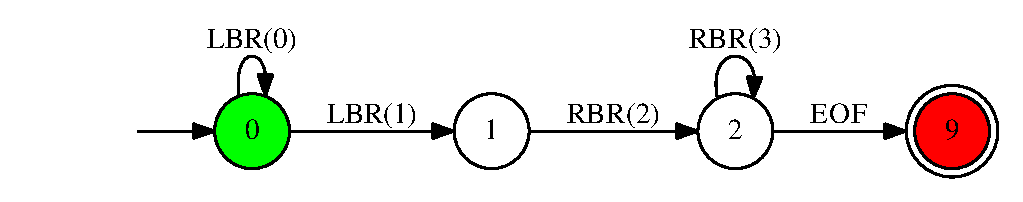
\includegraphics[scale=0.3]{dot/in3.eps}
   }  
   \hfill
    \subfloat[SPPF\label{resultSPPF}]{%
      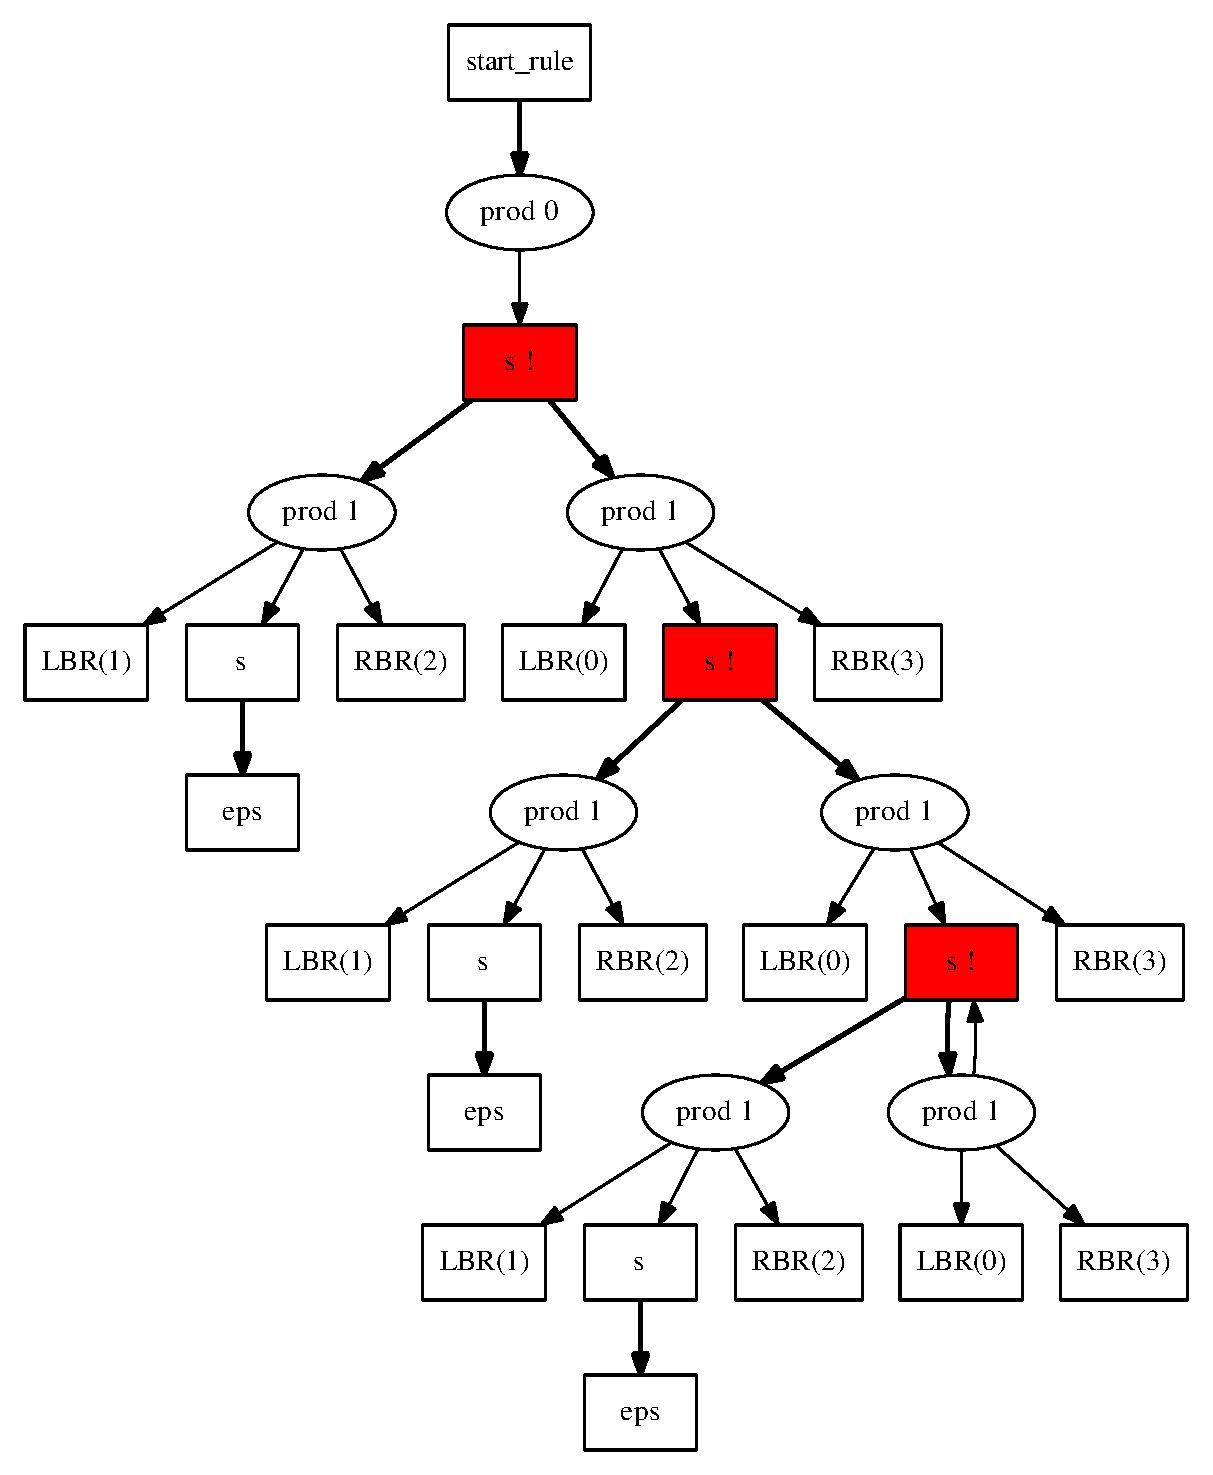
\includegraphics[scale=0.3]{dot/out3.eps}
    }
    \caption{Regular approximation and SPPF}
    \label{fig:SPPFforReg}
 \end{figure}

%\begin{figure}
%    \begin{center}
%        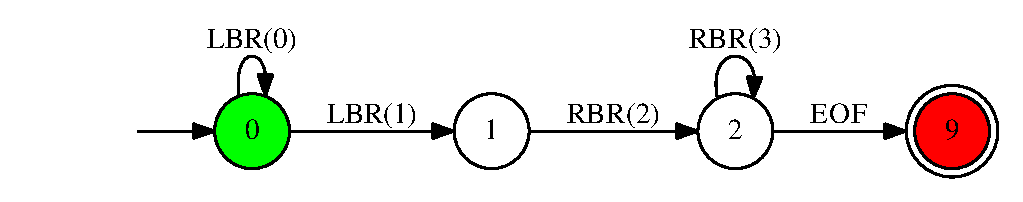
\includegraphics[scale=0.5]{dot/in3.eps}
%    \end{center}
%    \caption{$A_1$ -- input for our algorithm: regular approximation for string-embedded code after tokenization} 
%    \label{faApprox}
%\end{figure}

As it can be seen, some of the words from regular approximation do not belong to the reference language (for example, 
\verb|LBR LBR RBR|). The algorithm ignores such strings and constructs SPPF, which contains derivation trees 
for all recognized strings w.r.t. reference grammar.

%\begin{figure}
%    \begin{center}
%        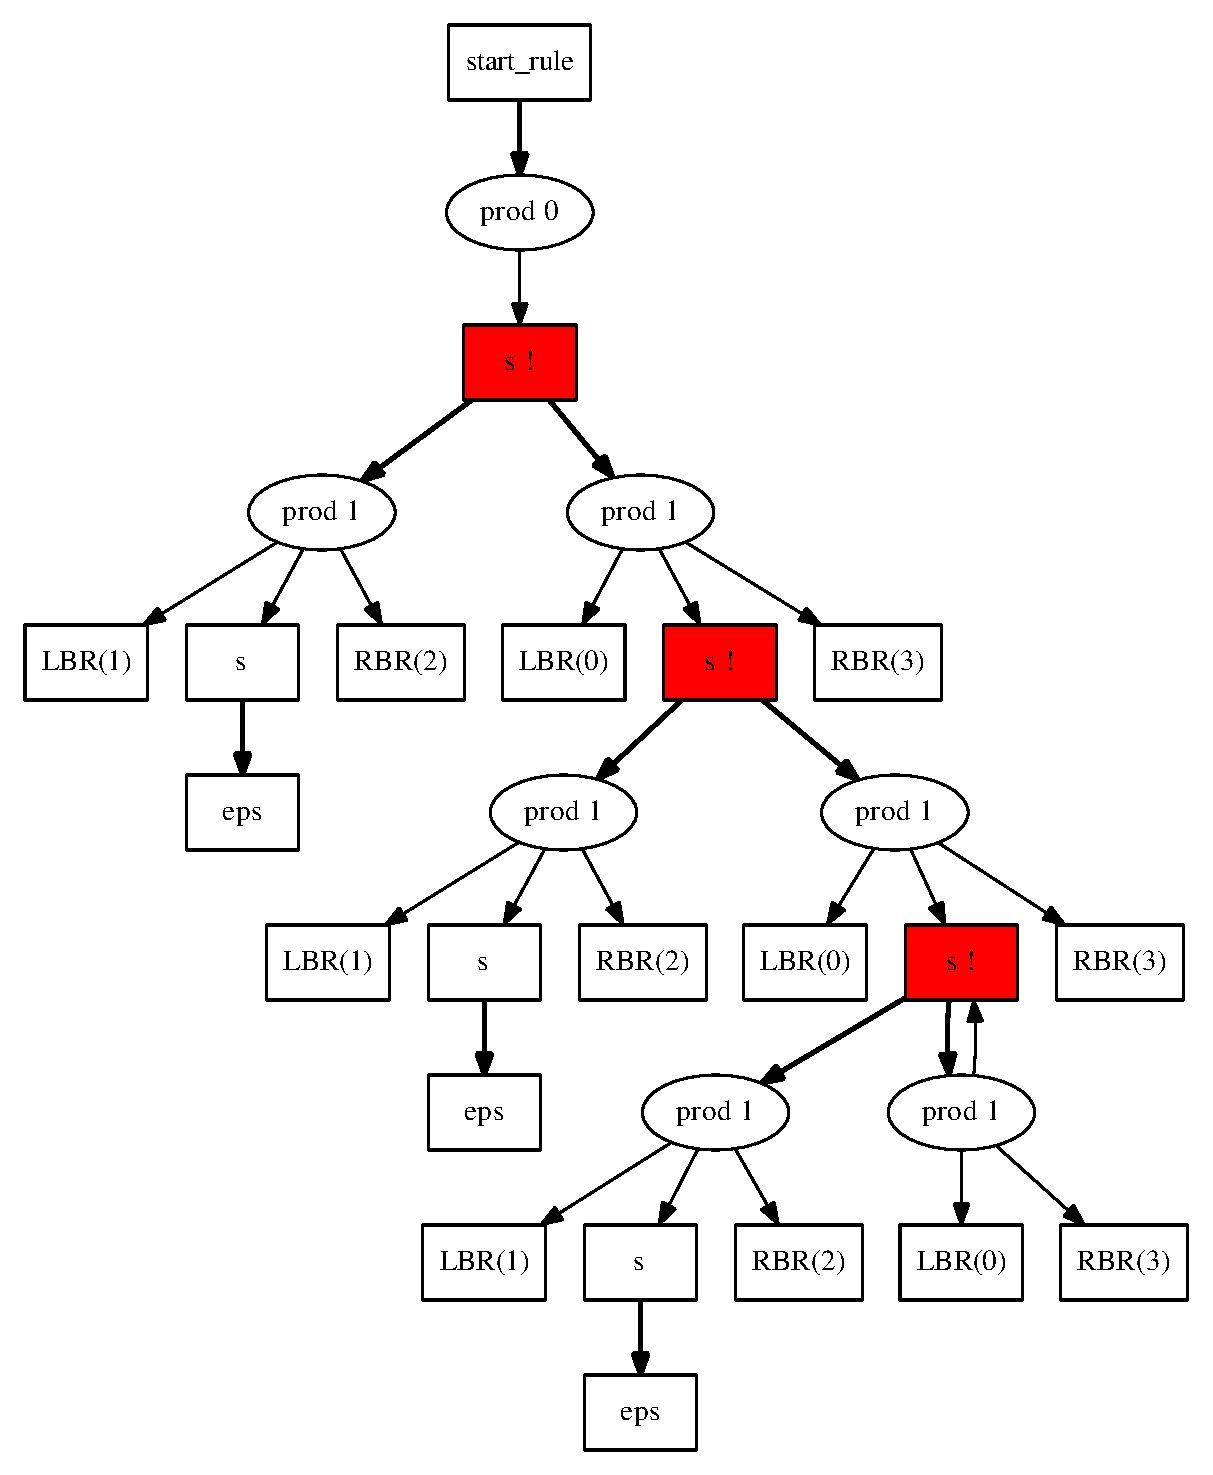
\includegraphics[scale=0.3]{dot/out3.eps}
%    \end{center}
%    \caption{SPPF for input FA presented in figure~\ref{faApprox}}
%    \label{resultSPPF}
%\end{figure}
\pagebreak
\section{\appendixname: RNGLR pseudocode}\label{RNGLRCode}

\begin{algorithm}[]
\begin{algorithmic}[1]
\caption{RNGLR algorithm}
\label{rnglr}
\Function{parse}{$grammar, input$}
  \State{$\mathcal{R} \gets \emptyset$} \Comment{Queue of tuples of GSS vertex, nonterminal, and reduction length}
  \State{$\mathcal{Q} \gets \emptyset$} \Comment{Collection of pairs of GSS vertex and parser state}
  \If{$input = \epsilon$}
    \If{$grammar$ accepts empty input} {report success}
    \Else { report failure}
    \EndIf
  \Else
    \State{\Call{addVertex}{$0, 0, startState$}}
    \ForAll{$i$ in $0..input.Length-1$}
      \State{\Call{reduce}{$i$}}
      \State{\Call{push}{$i$}}
    \EndFor
    \If{$i=input.Length-1$ and there is a vertex in the last level of GSS which state is accepting}
      \State{report success}
    \Else { report failure}
    \EndIf
  \EndIf
\EndFunction
\Function{reduce}{$i$}
  \While{$\mathcal{R}$ is not empty}
    \State{$(v, N, l) \gets \mathcal{R}.Dequeue()$}
    \State{find the set $\mathcal{X}$ of vertices reachable from $v$ along the path of length $(l-1)$}
    \State{or length $0$ if $l=0$}
    \ForAll{$v_{h} = (level_{h}, state_{h})$ in $\mathcal{X}$}
      \State{$state_{t} \gets$ calculate new state by $state_{h}$ and nonterminal $N$}
      \State{\Call{addEdge}{$i, v_{h}, v.level, state_{tail}, (l=0)$}}
    \EndFor
  \EndWhile
\EndFunction
\Function{push}{$i$}
  \State{$\mathcal{Q^{'}} \gets$ copy $\mathcal{Q}$}
  \While{$\mathcal{Q^{'}}$ is not empty}
    \State{$(v, state) \gets \mathcal{Q}.Dequeue()$}
    \State{\Call{addEdge}{$i, v, v.level + 1, state, false$}}
  \EndWhile
\EndFunction
\end{algorithmic}
\end{algorithm}

\begin{algorithm}[]
\begin{algorithmic}[1]
\caption{GSS construction}
\label{RNGLRMain}
\Function{addVertex}{$i, level, state$}
  \If{GSS does not contain vertex $v = (level, state)$}
    \State{add new vertex $v = (level, state)$ to GSS}
    \State{calculate the set of shifts by $v$ and the $input[i+1]$ and add them to $\mathcal{Q}$}
    \State{calculate the set of zero-reductions by $v$ and the $input[i+1]$ and}
    \State{add them to $\mathcal{R}$}
  \EndIf
  \State{\Return{$v$}}
\EndFunction
\Function{addEdge}{$i, v_{h}, level_{t}, state_{t}, isZeroReduction$}
  \State{$v_{t} \gets$ \Call{addVertex}{$i, level_{t}, state_{t}$}}
  \If{GSS does not contain edge from $v_{t}$ to $v_{h}$}
    \State{add new edge from $v_{t}$ to $v_{h}$ to GSS}
    \If{not $isZeroReduction$}
      \State{calculate the set of reductions by $v$ and the $input[i+1]$ and}
      \State{add them to $\mathcal{R}$}
    \EndIf
  \EndIf
\EndFunction
\end{algorithmic}
\end{algorithm}



\end{document}
